
Figure \ref{pipeline} summarizes the general methodology that will be discussed. We will focus
on three main components, Data collection, Data processing, and Data exploration.

\ \\ 
\noindent
\begin{tabular}{@{}cc}
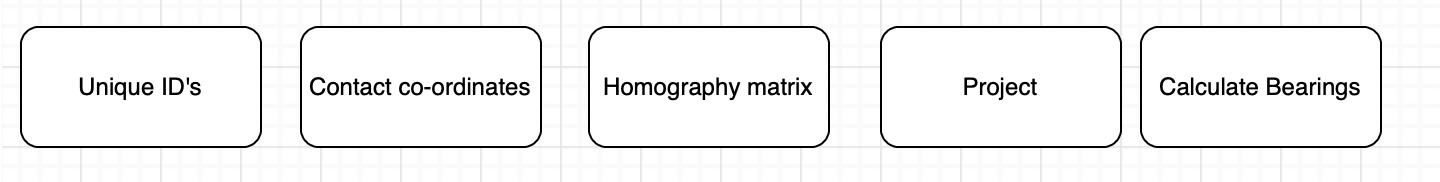
\includegraphics[width=1.0\columnwidth]{temp.png} 
\end{tabular}
\captionof{figure}{Data pipeline overview} 
\label{pipeline}

\subsection{Data Collection}

The Yrsas Plads junction in Copenhagen was chosen as the location for our primary data collection. 
This junction faces several challenges producing “conflicts, unsafe situations, illegal road user behavior and great dissatisfaction among road users at the intersection” \cite{CPHpost_2021}.
These challenges make the Yrsas Plads junction one of the more complicated junctions in Copenhagen and would serve as an excellent base for this quantitative analysis method. 
As this is a large junction, we have implemented a two cameras recording setup on the opposite side of the junction; this provides good coverage regardless of traffic obstructions.
\subsubsection{Recording Location}

There are three considerations to take into account when applying these methods to a junction.
\begin{itemize}
	\item Junction size
\end{itemize}
Larger junctions would require a two camera setup as detailed, but this might not be optimal for intersections much Larger
than the Yrsas Plads junction. A larger junction might require more cameras which will need some implmentation tweeks.
\begin{itemize}
	\item Camera mounting points
\end{itemize}
\begin{itemize}
	\item Junction composition
\end{itemize}

\subsubsection{Camera Selection}

Any camera device with a wide enough field-of-view (FOV) to image the selected intersection, can record at 720p (1280×720 resolution, or 1-megapixel), and that allows remote viewing of its interface,
will suffice. Having tested a Raspberry Pi recording setup (Raspberry Pi, camera external battery bank and an LCD screen case) we would not recomended a setup with self built hardware.
Although the Raspberry Pi setup meets the basic requirements mentioned earlier, the major issue is the usability of such a setup. There are unneeded complexities in
setting up the hardware and having a surety of its correct functioning when compared to alternatives that are built and optimized for video recordings such as
mobile phones or action cameras. Mobile phones and action cameras often offer methods of remote viewing of their interfaces that are much more
intuitive than what can be reasonably achieved with a Raspberry Pi setup, as these devices often have data connectivity and/or WIFI allowing for the use of remote control/viewing apps such as TeamViewer or in terms of action cameras
offer software applications that allow connecting to the camera for remote viewing. Being able to remotely view the camera interface is important when mounting the
camera and adjusting it's position to get a good view of the intersection.

\ \\
For these reason, we chose to use two mobile phones those being an LG G6 and a Samsung S7 Edge.
These devices offer wide enough FOV to record the parts of the junction we are interested in from the selected mounting locations, have high-resolution cameras, and allow for remote viewing over WIFI using TeamViewer.
FOV being the maximum area a camera can image. 
\ \\

A formal method of selecting a recording device would be to select one with a large enough FOV that can image the entire junction from the mounting position closest to the junction. Given a recording location, we can calculate the FOV needed using equation \ref{eq:1}.
If $\theta > FOV$, then the FOV is too small. 
\color{red}
Note: Label images and make them more understandable.
\color{black}

\begin{equation}
    \theta = tan^-1(\frac{\frac{width}{2}}{adjacent}) * 2\label{eq:1}
  \end{equation}

\ \\ 
\begin{figure}[h]
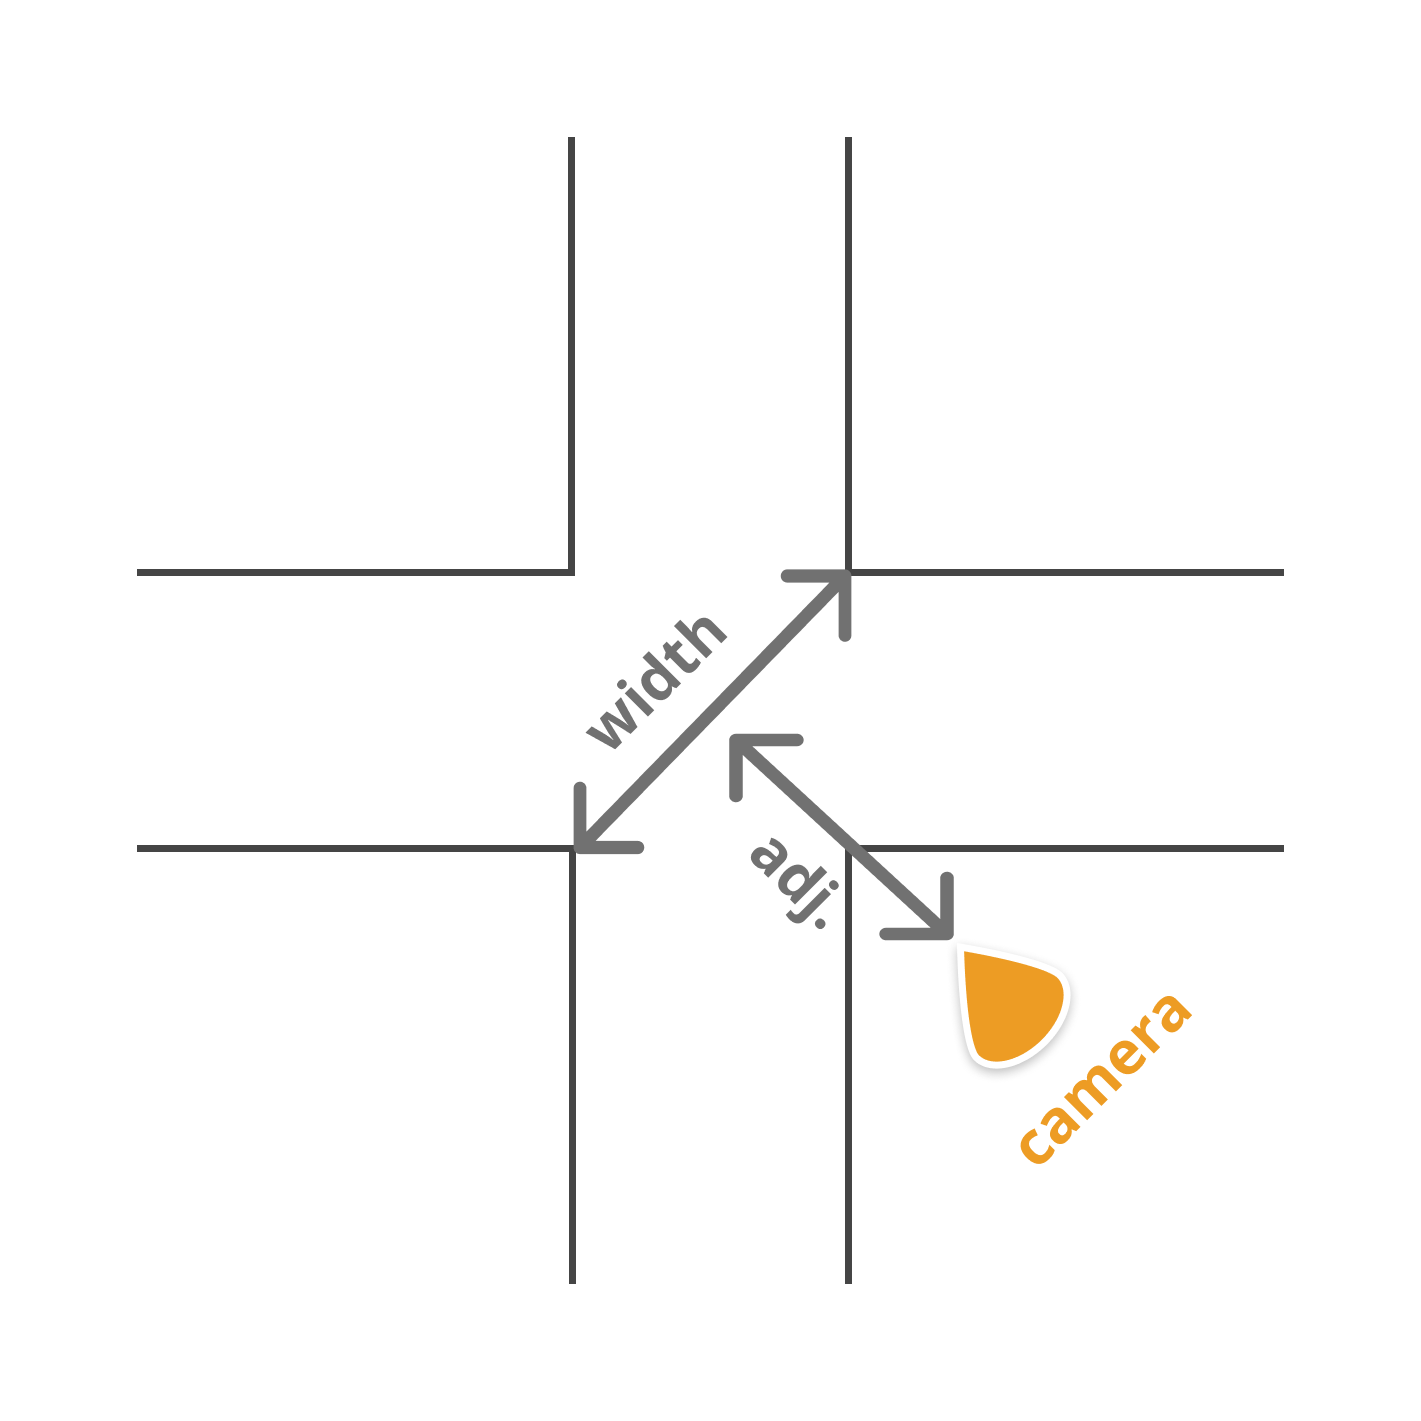
\includegraphics[scale=1.0]{location.png}
\centering 
\end{figure}
\captionof{figure}{Camera location}
\label{Camera location}

\ \\
Battery life and storage capacity should also be considered depending on the amount of intended recording. 
With regards to storage, a good estimate for video size would be 149MB per 1 min of FullHD (1920*1080) at 30FPS. Storage should be selected
with the intended amount of recording time.

\subsubsection{Camera mounting}

As we chose mobile phones to record with we had access to a wide variety of mobile phone mounts on store such as Amazon.
To mount the Samsung S7 Edge we used a flexible arm mount and for the LG G6, we used a custom-made mounting system.
The method of mounting a camera is very much dependant on where the camera is placed and on what. For example, the Samsung S7 Edge's
mounting location was easily accessible and therefore we could simply clamp the system onto a pole. Whereas the LG G6's location was relatively 
high off the ground and unreachable, therefore we created a mount that allowed us to use an extendable arm to hook the camera onto the position.

For best results, the cameras should be set up as parallel to the road's surface as possible and high up enough not to have the FOV obstructed by obstacles.
A minimum angle of 30° downwards and a minimum height of 2 meters is recommended.

Note: Picture of our locations and mounting system.

\subsection{Data Processing}

\ \\ 
\noindent
\begin{tabular}{@{}cc}
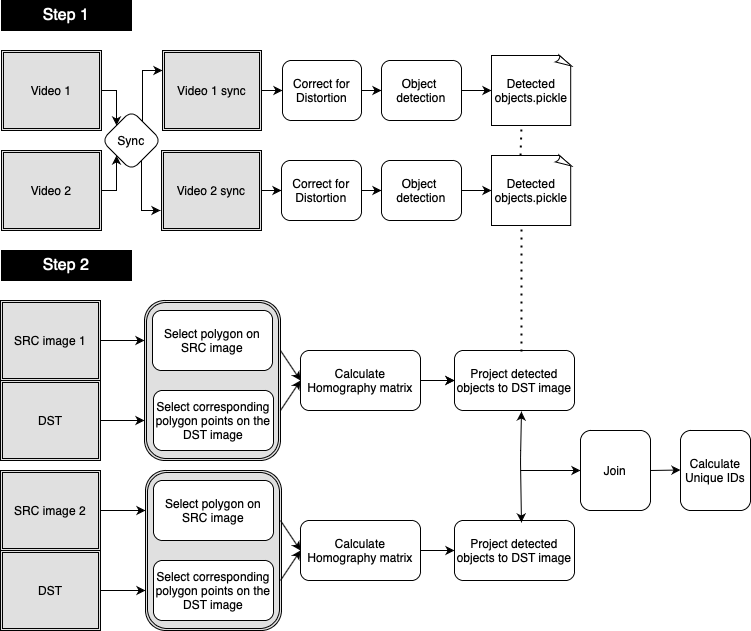
\includegraphics[width=1.0\columnwidth]{data_flow.png} 
\end{tabular}
\captionof{figure}{Data Pipeline}
\label{data}


Figure \ref{data} offers a general overview of the data processing steps. No special hardware is required, but a CUDA-enabled GPU is optimal for object detection using YOLO.
\ \\
\subsubsection{Distortion Correction}

Cameras often suffer from optical aberration where straight lines appear bent. This can be observed on wide-angle camera lenses such as that of the LG G6 used in this study.
The specific type is \textit{positive radial distortion} as shown in figure \ref{distortion}, with lines curving outwards in a barrel shape.
Another form of radial distortion is \textit{pincushion distortion} with lines bend towards the center of the image. These aberrations are a result 
of the curved shape of the camera lens.

\ \\ 
\begin{figure}[h]
  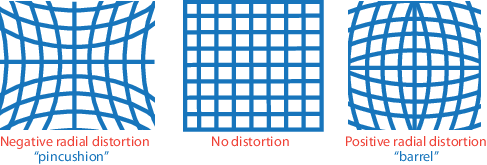
\includegraphics[scale=0.65]{calibration_radial_distortion.png}
  \centering 
  \end{figure}
  \captionof{figure}{Distortion}
  \label{distortion}

\ \\

There is also a possibility of further distortion if the camera sensor and the lens are not parallel, also known as \textit{tangential distortion}.
Ideally, there should be no radial nor tangential distortion.
\ \\
Distortion can lead to incorrect projection and therefore joining of video sources later on.
To correct for this we make use of OpenCVs \cite{noauthor_opencv/opencv_2021} camera calibration toolbox.

\color{red}
In order to correct for distortion, we need to find the camera matrix and distortion coefficients... Explain the maths a bit more.
\color{black}
\ \\
\subsubsection{Object Detection}

The raw video is output as a MPEG-4 file. This video file is fed to YOLOv5 for object detection. YOLO, \textit{You Only Look Once},
is a real-time object detection algorithm. YOLOv5 is trained on the COCO dataset \url{https://cocodataset.org}, which comprises over 330,000 thousand images
with over 1,5 million objects in over 80 object classes.
\ \\ 
YOLO is well known for its real-time speed, and accuracy \cite{redmon2016look}.
\ \\ 
At the most basic level, YOLO resizes an input image, runs a single convolutional network on the resized image
and then thresholds the resulting detections by the model’s confidence.
\ \\ 
Predicted objects are represented as bounding boxes with the output being represented as $[[frame id][xmin][ymin][xmax][ymax][confidence]]$
\ \\
The min and max values for x and y represent a bounding box for the identified bicycle.

\subsubsection{Homography Matrix}

A homography matrix is a transformation matrix between two planes \cite{hartley_zisserman_2004}. It can be used to perform a perspective transformation of a plane from a source image $P(x_r, y_r)$ onto a plane on a destination image $Q(x_i, y_i)$.
The source image in our case is the plane of the road surface from the recorded video at the intersection to the road surface from an aerial view of the same intersection.  
This will allow us to view the cyclist movements from an aerial view.
\ \\ 
\begin{figure}[h]
  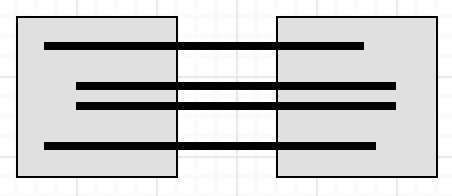
\includegraphics[scale=1.0]{Homography_proj.png}
  \centering 
  \end{figure}
  \captionof{figure}{SR to DST}
  \label{homography}
\ \\ 
To calculate the homography matrix, we need to solve the for the system of linear equations, $P = HQ$,
\ \\
$P$ being points in a polygon on the source image, $Q$ the corresponding polygon on the destination image $H$ being the homography matrix.
\begin{align}
\label{eq:3}
  \begin{bmatrix}
    x_{i} \\
    y_{i} \\
    z_{i} \\
  \end{bmatrix}
  &= \begin{bmatrix}
      h_1 & h_2 & h_3 \\
      h_4 & h_5 & h_6 \\
      h_7 & h_8 & h_9 \\
  \end{bmatrix}
  \begin{bmatrix}
    x_{r} \\
    y_{r} \\
    z_{r} \\
  \end{bmatrix}
\end{align}

\subsubsection{Projection}

Before we can project the cyclist onto an aerial view, we first need to calculate the 2D coordinates of their contact points with the road surface.
Given \ref{representation} we can calculate this by the following

$$x = xmin + \frac{(xmax - xmin)}{2}$$
$$y = ymin$$
\
Using the homography matrix, we can now project the contact points $(x, y)$ of the cyclist onto the destination
image. This is achieved by applying $z$ to each point as a constant to create $Q(x_i, y_i, 1)$ and then we multiply it by the homography matrix. 

\subsubsection{Merging Sources}

To merge the data from the two video sources, we take a naive approach. For optimal coverage, the cameras are set up on
opposite sides of the junction. We simply cut the video sources in half along the mid-point between
the two cameras along the junction to join them. The data is then merged.

\subsubsection{Multiple object tracking}

In order to connect observations into trajectories of individual cyclist, we apply 
simple online and real-time tracking algorithm, SORT \cite{abewley_abewley/sort_2021}, as initially described in \cite{Bewley2016_sort}. 
SORT aims to address multiple object tracking (MOT) where object across frames needs to be connected. 
\color{red}
Note: Explain more about SORT predict bbox then IOU for actualy bbox.
\color{black}
\ \\
We assume arbitrary bounding box dimensions of 10*10 pixels for the projected cyclists to join the tracks from multiple sources. 
Passing the algorithm the bounding boxes per frame, we get a unique ID associated with each observation.

\subsection{Data Exploration}

There are two objectives for the data exploration, those being:
\begin{itemize}
	\item Desire path discovery
	\item Alert Zones - For behaviour observations and counts
\end{itemize}

\subsubsection{Rainbow Tracks}

A method of desire path discovery.

\ \\ 
\noindent
\begin{tabular}{@{}cc}
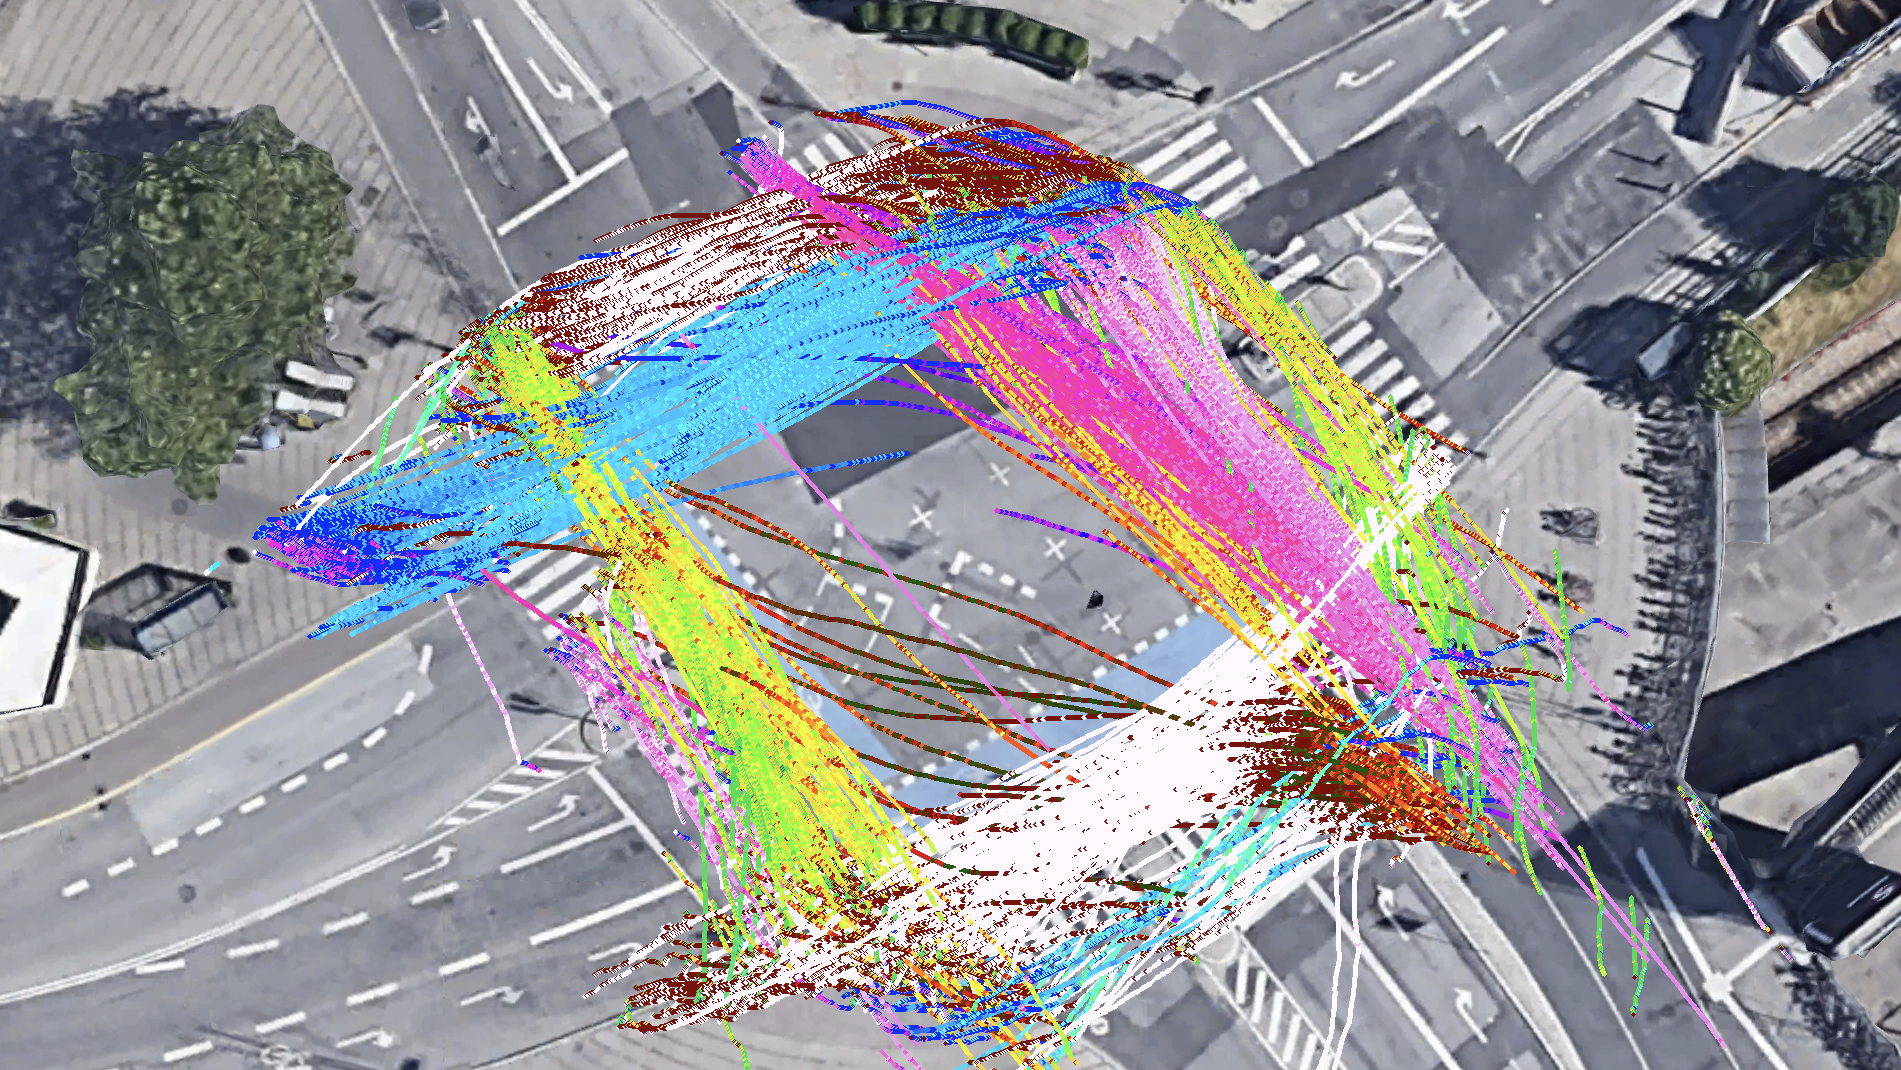
\includegraphics[width=1.0\columnwidth]{rainbow.png} 
\end{tabular}
\captionof{figure}{Rainbow}
\label{Rainbow}
\ \\

To find aggregated desire lines from the data we took an approach which we call "Rainbow tracks". This involves coloring tracks by the bearing between consecutive points in each trajectory. After calculating the bearing, we then get a color from a gradient color wheel. This approach has the added benefit of encoding direction into 
each track.
Note: Maybe just an equation demonstrating the bearing calculation.
\ \\ 

\begin{equation}
  UniqueID_i = [(x_1, y_1)...(x_a+1, y_a+1)]\label{eq:3}
\end{equation}

\subsubsection{Alert Zones and Counts}

\color{red}
We created a "Tool name" that allows the definition of specific areas as "red zones". These zones provide us with easy reference to activity in the zones throughout the videos.
Using these zones, we can count cyclist and observe their behavior at points on the junction that might be difficult or
problematic.

Note: Picture of interface?
